\documentclass[10pt,a4paper]{article}
\usepackage[utf8]{inputenc}
\usepackage{amsmath}
\usepackage{amsfonts}
\usepackage{amssymb}
\usepackage{natbib}
\usepackage{graphicx}

\title{XOR single-layer model theory}
\author{Max Cotton}
\date{}

\begin{document}

\maketitle

\section{Setup}

\begin{figure}[h!]
\centering
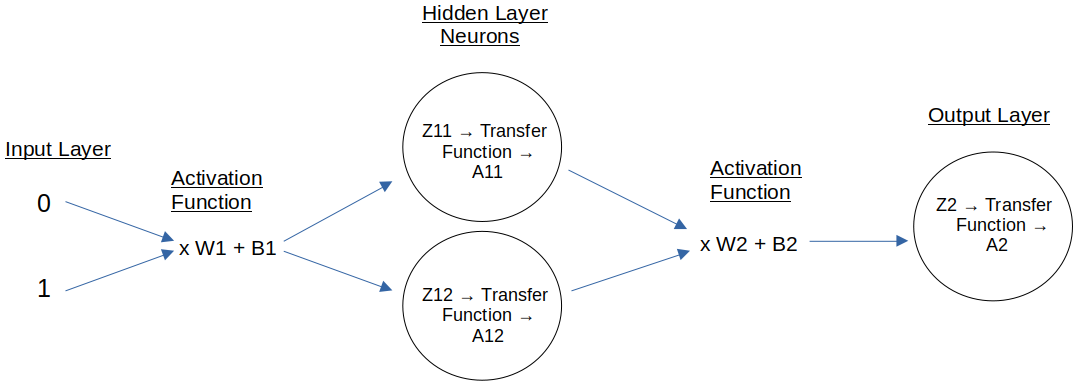
\includegraphics[width=1\textwidth]{src/images/xor-ann-diagram.png}
\end{figure}

\begin{itemize}
    \item Where the weights W11, W12, W21 and W22 are together in an array W1, as the hidden weights, initially given random values
    \item Weights W3 and W4 are together in array W2, as the output weights
    \item Z11 and Z12 are together in an array Z1, and is the dot product of the W1 array and the input array (X)
    \item A11 and A12 are together in an array A1, and is sigmoid(Z1)
    \begin{itemize}
        \item Where $sigmoid(Z) = \frac{1}{1+e^{-Z}}$
    \end{itemize}
    \item Z2 is the dot product of the W2 array and A1
    \item A2 is sigmoid(Z2), which is the prediction Y
\end{itemize}

\section{Forward Propagation}
For each epoch the input array consisting of a combination of a 0 and/or 1, is fed through the network to obtain a prediction Y

\section{Back Propagation}

\begin{itemize}
    \item Once a prediction is obtained, you then move back through the network adjusting the weights
    \item The "Cost" (how wrong the prediction is) can be calculated with the cost function, which calculates the average squared difference between the prediction and the actual values. This shows how well the network is performing.
    \begin{itemize}
        \item Where $Cost = -(\frac{1}{nInputs}) * \sum(Y * log(A2) + (1-Y) * log(1-A2))$
    \end{itemize}
    \item Weights are adjusted via Gradient Descent, which aims to get the minimum cost value, with the following formula:
    \begin{itemize}
        \item $W = W - learningRate * \frac{\partial{L}}{\partial{W}}$
        \item Where $\frac{\partial{L}}{\partial{W2}} = (A2-Y) * A1$
        \item And $\frac{\partial{L}}{\partial{W1}} = X * A1 * (1-A1) * W2 * (A2-Y)$
    \end{itemize}
\end{itemize}

\section{Derivations for $\frac{\partial{L}}{\partial{W2}}$ and $\frac{\partial{L}}{\partial{W1}}$}

\end{document}